% 05 · Modelling — hand-written LaTeX edition of 05-modelling.md
%
%   xelatex -output-directory=_pdf docs/05-modelling.tex   (run twice, for \ref and the ToC)
%
% This is what the chapter looks like when LaTeX is the source rather than a
% conversion target: real theorem environments, automatic section numbering,
% and § cross-references that renumber themselves.

\documentclass[11pt]{article}

\usepackage{fontspec}
\usepackage{unicode-math}
% TeX Gyre Pagella is the free Palatino, and Pagella Math is its matching
% math companion — text and formulas then share one design.
\setmainfont{texgyrepagella}[
  Extension      = .otf,
  UprightFont    = *-regular,
  BoldFont       = *-bold,
  ItalicFont     = *-italic,
  BoldItalicFont = *-bolditalic ]
\setmathfont{texgyrepagella-math.otf}

\usepackage[margin=1.1in]{geometry}
\usepackage{amsmath, amsthm}   % not amssymb: unicode-math supplies it and they collide
\usepackage{booktabs, tabularx, array}
\usepackage{graphicx}
\usepackage{enumitem}
\usepackage{microtype}
\usepackage[dvipsnames]{xcolor}
\usepackage[colorlinks=true, linkcolor=MidnightBlue, urlcolor=MidnightBlue]{hyperref}

\graphicspath{{figures/}}
\linespread{1.1}
\setlist{itemsep=0.3em, topsep=0.5em}

% --- Labelled entries -------------------------------------------------------
% Run-in, bold label, unnumbered — the markdown convention, kept deliberately.
% CLAUDE.md bans Def 1.1-style numbering and the ∎, so both are switched off.
\newtheoremstyle{runin}
  {0.8em}{0.8em}{}{}{\bfseries}{.}{ }{}
\theoremstyle{runin}
\newtheorem*{definition}{Definition}
\newtheorem*{claim}{Claim}
\newtheorem*{note}{Note}
\newtheorem*{example}{Example}
\renewcommand{\qedsymbol}{}

% A pointer at another chapter. In the markdown these are live links; in a
% standalone PDF they can only be a citation, so they are set as one.
\newcommand{\ch}[2]{\textsc{ch.~#1}~\textit{#2}}

\newcolumntype{L}[1]{>{\raggedright\arraybackslash}p{#1}}

% An empty checkbox, drawn rather than taken from a font, so it never depends
% on the main face carrying U+25A1.
\newcommand{\tickbox}{\framebox[0.8em]{\rule{0pt}{0.62em}}}

\title{\textbf{05 · Modelling}}
\date{}
\author{}

\begin{document}
\maketitle
\vspace{-3em}
\tableofcontents
\bigskip

% ============================================================================
\section{Why one split is not a backtest}
\label{sec:one-split}

\subsection{The textbook split}

\begin{definition}[Split]
A \emph{split} cuts the sample by date into three contiguous blocks: \textbf{train}, on which
coefficients are estimated; \textbf{validation}, on which choices between fitted models are made;
and \textbf{test}, which is scored once and never chosen on.
\end{definition}

\begin{figure}[h]
  \centering
  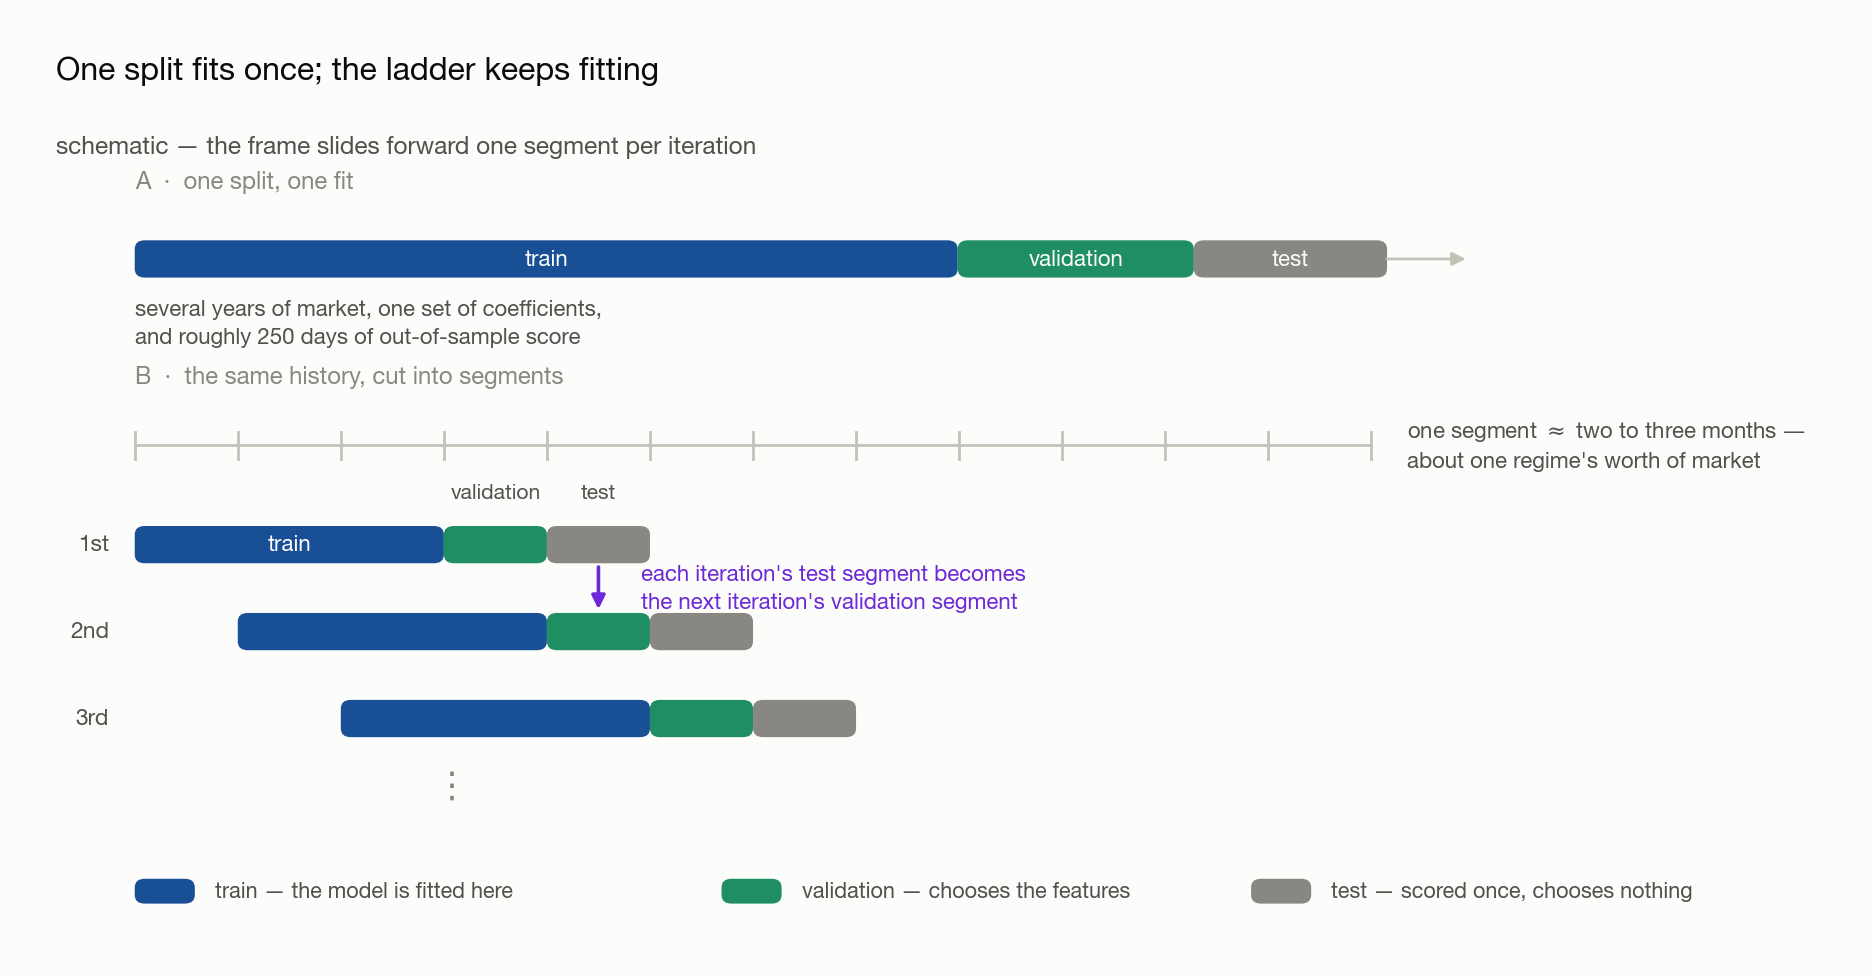
\includegraphics[width=\linewidth]{split-vs-ladder-light}
\end{figure}

The order matters and is not a convention: the blocks run forward in time, because a model that
was fitted on next year and scored on last year has learned something no live book could have
known.

\subsection{What the single split costs}
\label{sec:defects}

Three defects, and they compound.

\begin{center}
\begin{tabularx}{\linewidth}{@{}L{3.4cm}X@{}}
\toprule
\textbf{Defect} & \textbf{What goes wrong} \\
\midrule
One fit discards time
& A single set of coefficients over several years asserts that those years were one market. Early
in the pandemic the world locked down at once and nobody wanted oil; the consensus was that demand
had permanently moved online. It had not --- the economy reopened, and energy then flew on war. A
coefficient estimated across both states describes neither. \\
\addlinespace
Almost nothing is left to score
& Give validation a year and test a year and validation is roughly 250 dates. A year is also too
little market: the regimes it contains are whichever ones happened to fall inside it, so the split
never asks what the strategy does when the regime turns. A maximum drawdown measured over one calm
year is not a risk estimate. \\
\addlinespace
The sample is small and the signal is faint
& A school dataset with a thousand points and an $R^2$ of 0.5 is ordinary, and in physics 0.9 is
ordinary. In finance \textbf{0.1 to 0.2 is already a good $R^2$} --- see \ch{09}{IC and $R^2$}.
Weak true dependence plus few observations is precisely the regime in which a fit lands on noise:
a line through ten points drawn from a cloud reaches $R^2$ 0.8 easily. \\
\bottomrule
\end{tabularx}
\end{center}

\subsection{The fix that is not one}
\label{sec:duplication}

\begin{claim}
Duplicating the sample changes no coefficient, and inflates every $t$-statistic by roughly
$\sqrt{2}$.
\end{claim}

\begin{proof}
Write the fit as $b = (X^{\mathsf{T}} X)^{-1} X^{\mathsf{T}} y$, with $X$ the $n \times p$ matrix
of signal values, $y$ the forward returns, and $b$ the estimated coefficients. Stacking the sample
twice gives $X_2^{\mathsf{T}} X_2 = 2 X^{\mathsf{T}} X$ and
$X_2^{\mathsf{T}} y_2 = 2 X^{\mathsf{T}} y$, so
\[
  b_2 = \left(2 X^{\mathsf{T}} X\right)^{-1} 2 X^{\mathsf{T}} y = b\,.
\]
The residuals repeat as well, so the residual sum of squares doubles while the degrees of freedom
go from $n - p$ to $2n - p$; for $n$ large the variance estimate $s^2$ is therefore essentially
unchanged. But the reported covariance is
$s^2 (X_2^{\mathsf{T}} X_2)^{-1} = s^2 (X^{\mathsf{T}} X)^{-1} / 2$ --- halved. Standard errors
fall by $\sqrt{2}$ and $t$-statistics rise by the same factor, on evidence that never arrived.
\end{proof}

\begin{note}
This is the standard interview question, and the reason it is asked is that people reach for it.
Manufacturing rows is overfitting with extra steps; the answer to too few observations is to score
more of the ones you have, which is \S\ref{sec:ladder}.
\end{note}

% ============================================================================
\section{The walk-forward ladder}
\label{sec:ladder}

\subsection{How long a segment should be}

\begin{definition}[Segment]
A \emph{segment} is a short contiguous block of dates --- here \textbf{two to three months} ---
treated as one regime.
\end{definition}

The length is set by how fast the market can change its mind, and the market is made of people.
Within a day a regime shift is implausible: individuals change their view constantly, the crowd
does not. Within a month, after a run of large news, one shift is plausible. Within a year or two
there is room for several, because that is enough time for the same participants to change their
minds repeatedly. So a segment must be short enough that one segment is approximately one regime,
and long enough to hold a usable sample.

\subsection{The slide}

Cut the history into segments $1, 2, 3, \ldots$ and slide a frame across them:

\begin{center}
\begin{tabular}{@{}cccc@{}}
\toprule
\textbf{Iteration} & \textbf{Train} & \textbf{Validation} & \textbf{Test} \\
\midrule
1 & 1--3 & 4 & 5 \\
2 & 2--4 & 5 & 6 \\
3 & 3--5 & 6 & 7 \\
\bottomrule
\end{tabular}
\end{center}

\begin{claim}
The ladder repairs all three defects of \S\ref{sec:defects} at once.
\end{claim}

Each fit now sees one regime's worth of data and is re-estimated as the market moves on, so time
is no longer averaged away. Every segment past the first frame is eventually scored out of sample,
so the out-of-sample record grows with the length of the history instead of being fixed at one
year. And a regime shift that lands inside a validation segment is now a \emph{test} the strategy
has to pass, rather than an event the single split happened to miss.

\begin{note}
Read the table down its two right columns: \textbf{each iteration's test segment is the next
iteration's validation segment.} Nothing is discarded between rungs, and no segment is ever scored
twice under the same coefficients.
\end{note}

\subsection{One rung, in full}
\label{sec:rung}

A rung is not a single fit. Train ends, a validation segment intervenes, and only then does test
begin --- so a model fitted on train alone is asked to predict across a gap of market it has never
seen, and pays for it.

The repair is the two-step shape that Lasso already imposes. Lasso adds an $L_1$ penalty to the
least-squares objective,
\[
  \min_{\beta} \quad \sum_t \left( y_t - \sum_j \beta_j x_{j,t} \right)^{2}
  \;+\; \lambda \sum_j \lvert \beta_j \rvert
\]
where $y_t$ is the forward return on date $t$, $x_{j,t}$ signal $j$'s value on that date,
$\beta_j$ its coefficient, and $\lambda \geq 0$ the penalty strength. The penalty drives
coefficients exactly to zero, which makes it a \textbf{feature selector}; and because the
surviving coefficients are biased toward zero by that same penalty, the standard practice is to
\textbf{refit} the survivors without the penalty before predicting.

\begin{figure}[h]
  \centering
  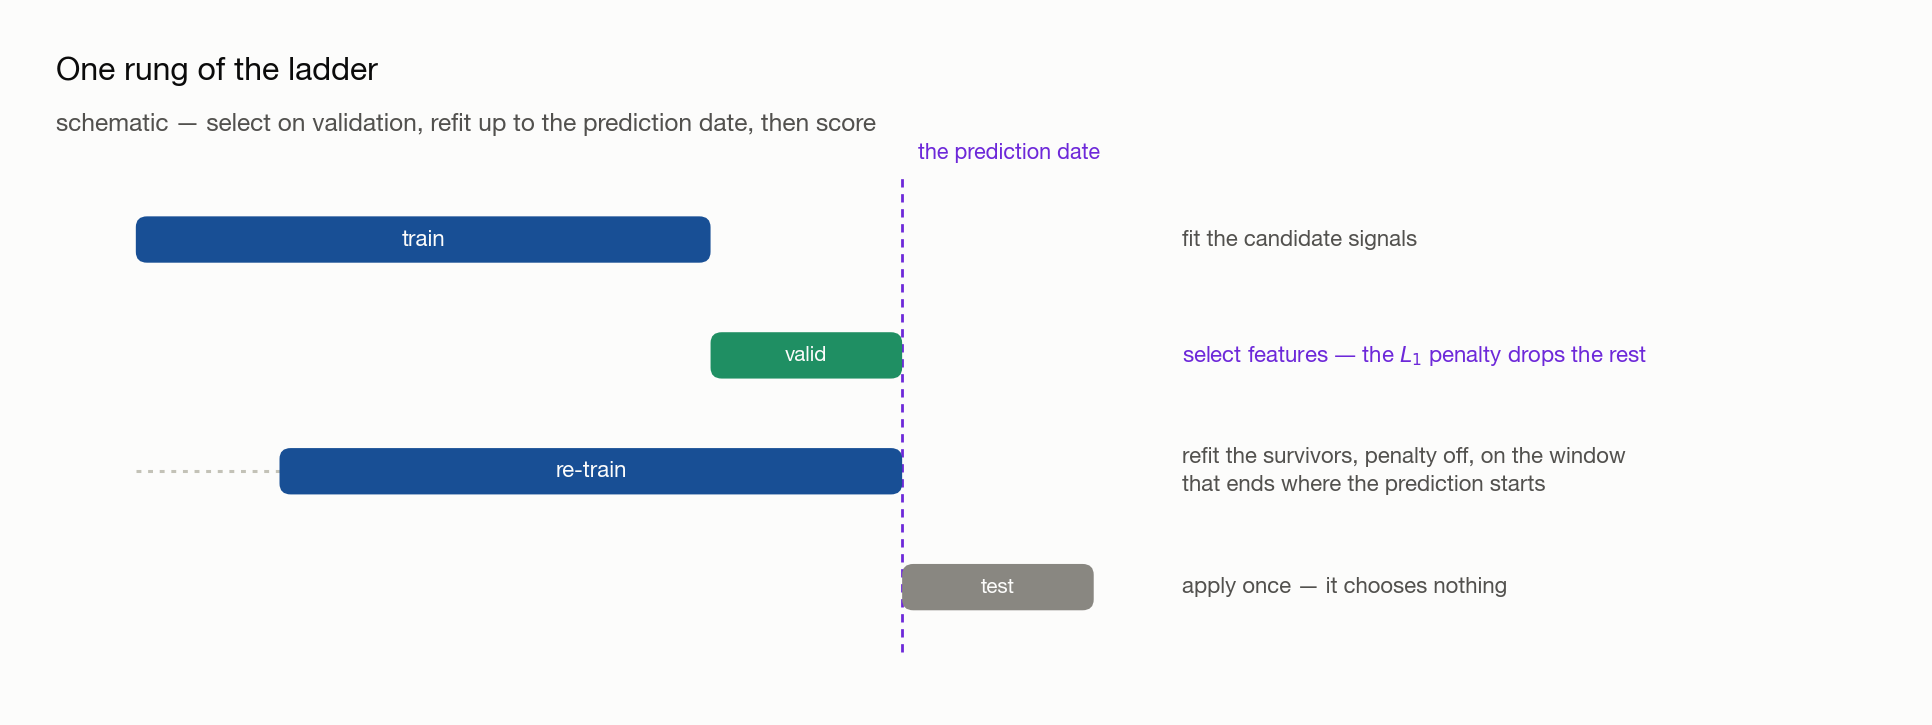
\includegraphics[width=\linewidth]{fold-anatomy-light}
\end{figure}

So each rung runs: \textbf{fit on train}, \textbf{select features on the validation segment},
\textbf{refit the survivors on a window ending where the prediction starts}, \textbf{apply once to
test}.

\begin{note}[Two house styles]
The refit window is either the training window shifted forward, or the training window plus the
validation segment. The sample sizes differ little and both are used in industry; it is a
preference, not a correctness question. What is not optional is that the window ends at the
prediction date --- see \S\ref{sec:lookahead}.
\end{note}

% ============================================================================
\section{Two validation layers}

The validation \emph{segment} inside each rung and the large held-out validation \emph{block} at
the end of the history are different objects with different powers.

\begin{figure}[h]
  \centering
  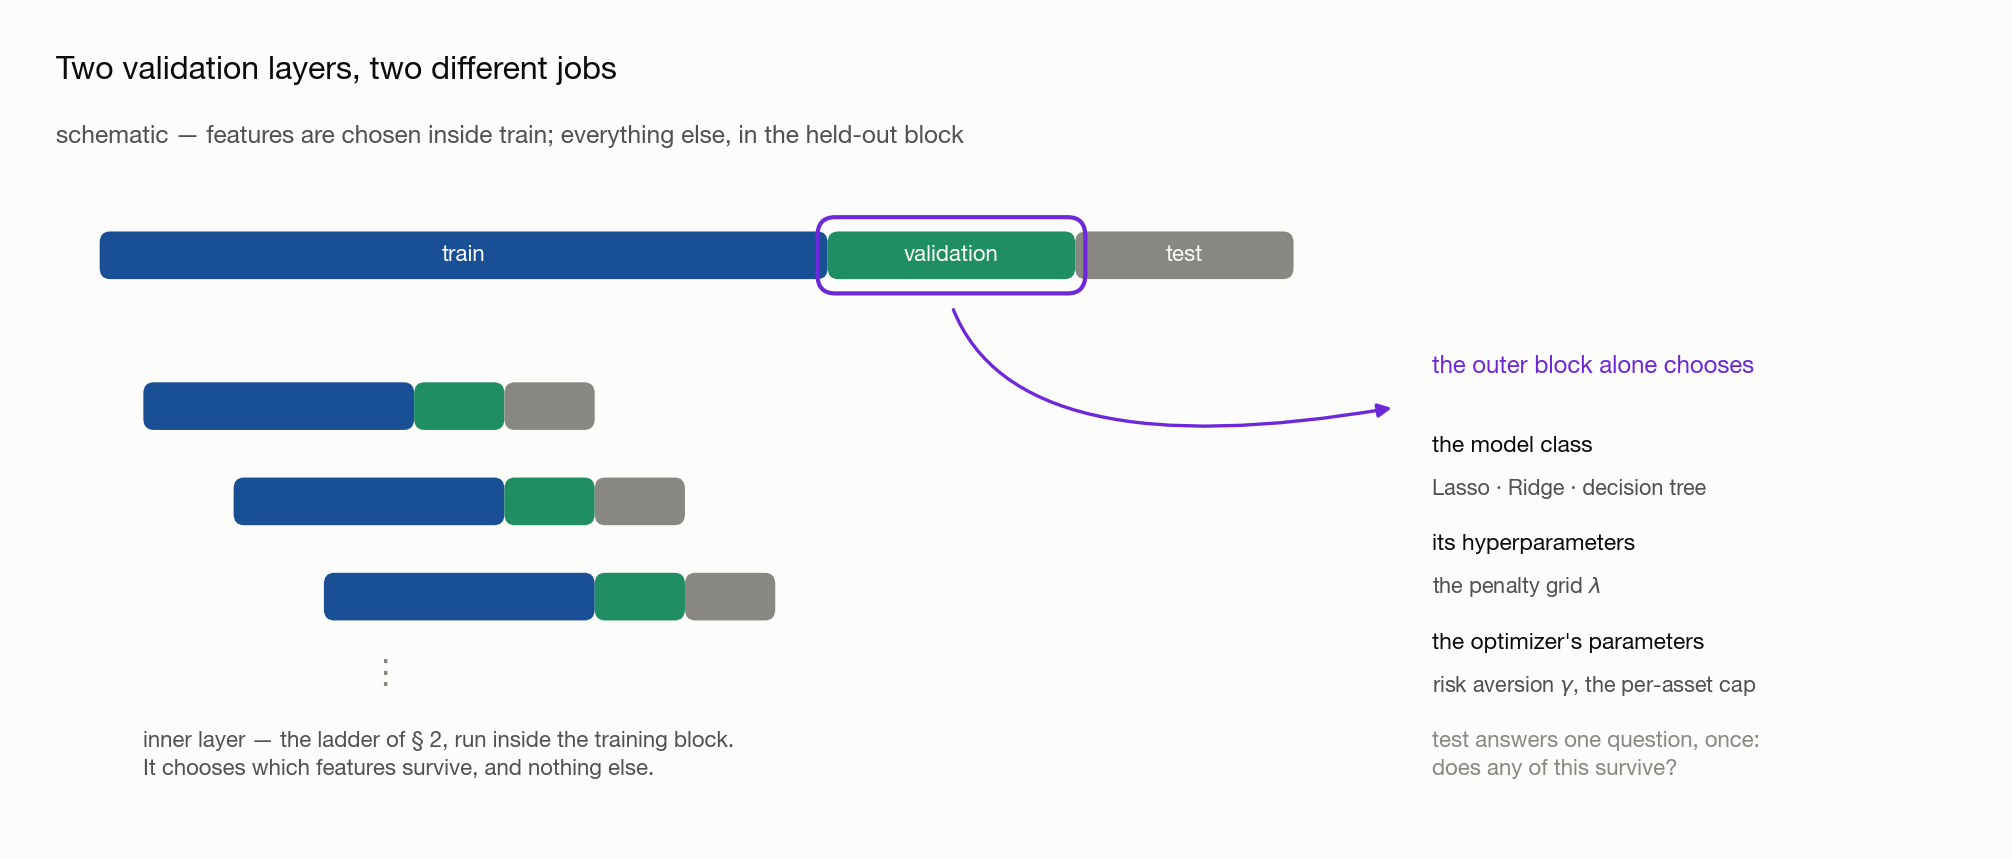
\includegraphics[width=\linewidth]{outer-validation-light}
\end{figure}

\begin{center}
\begin{tabularx}{\linewidth}{@{}L{3.6cm}XL{4.2cm}@{}}
\toprule
\textbf{Layer} & \textbf{May choose} & \textbf{May not} \\
\midrule
\textbf{Inner} --- the validation segment inside each rung
& which \textbf{features} survive, and the refit that follows
& anything held constant across rungs \\
\addlinespace
\textbf{Outer} --- the held-out validation block
& the \textbf{model class}, its \textbf{hyperparameters} ($\lambda$), and the \textbf{optimizer's
parameters}
& coefficients --- those are fitted on train \\
\addlinespace
\textbf{Test} & nothing & everything \\
\bottomrule
\end{tabularx}
\end{center}

\subsection{Why the inner layer cannot be skipped}

Exploration already looked at which signals worked \emph{in the training period}. Of course the
fit then describes that period well: momentum was selected partly because it was seen to work
there. That says nothing about whether it was useful going in, and the only way to find out is to
select on dates the selection did not see --- which is what the validation segment is for.

\begin{note}
A signal's usefulness is not a constant either. When more signals enter the book, or when one
starts to fail, momentum should no longer carry the weight it carried alone. Because the ladder
re-selects at every rung, that adjustment happens on its own rather than being asserted once.
\end{note}

\subsection{What only the outer block may decide}

$\lambda$ is not fitted, it is searched: run the ladder once per value on a grid --- 0.1, 0.5,
0.7, 1 --- and compare. The same is true of the model class itself (Lasso, Ridge, a decision
tree). Both comparisons need dates that no rung of the ladder consumed, which is exactly what the
held-out block is.

\subsection{The optimizer's parameters}
\label{sec:optimizer}

The prediction is not yet a portfolio. Weights come from a mean--variance problem: choose $w$ to
\[
  \max_w \quad E[r_p] - \gamma \cdot \mathrm{Var}[r_p]
\]
subject to constraints such as
\[
  \sum_i w_i = 1.0 \qquad \sum_i \lvert w_i \rvert \leq 2.0 \qquad \lvert w_i \rvert \leq 0.20
\]
--- net exposure 100 percent, gross exposure at most 200 percent, and no single asset above 20
percent --- where $w_i$ is the weight on asset $i$, $E[r_p]$ and $\mathrm{Var}[r_p]$ the
portfolio's expected return and variance, and $\gamma \geq 0$ the \textbf{risk-aversion
coefficient}.

Two of these are free parameters, and neither can be reasoned to:

\begin{itemize}
  \item \textbf{$\gamma$.} Nobody can say from first principles whether a risk appetite is 0.3,
    0.5 or 1. The number has no interpretable units --- it is a trade rate between two quantities
    measured in different things --- so it is chosen by running the grid and reading the result.
  \item \textbf{The per-asset cap.} With 37 assets, a 20 percent cap may be too tight for the book
    to hold enough of whichever names are paying; 25 or 30 percent may be the right ceiling. Gross
    and net exposure, by contrast, are set by mandate and are not tuned.
\end{itemize}

\begin{note}
All of this tuning belongs in the \textbf{outer} block. Tuning $\gamma$ inside the rungs would let
a portfolio parameter be chosen on the same dates the features were chosen on, and the held-out
block would then be measuring a strategy that had already been fitted to it.
\end{note}

% ============================================================================
\section{Preparing a signal for a model}

Two transformations stand between a raw signal and a model, and both exist to stop the fit from
tracking things that are not the market.

\subsection{Clipping: keep the observation, cap the value}
\label{sec:clip}

\begin{claim}
A ranked signal does not fill its range evenly --- the mass piles at both ends --- and those ends
move the fit far more than their count suggests.
\end{claim}

The first half is empirical: momentum in particular pins at an extreme whenever a name runs, so
the histogram is a barbell rather than a plateau. The second half is mechanical. In a
least-squares fit each observation's pull on the slope grows with its distance from the mean of
$x$, so a handful of far points can swing a coefficient that hundreds of central points barely
move. The coefficient then jumps for reasons that have nothing to do with the market.

\begin{figure}[h]
  \centering
  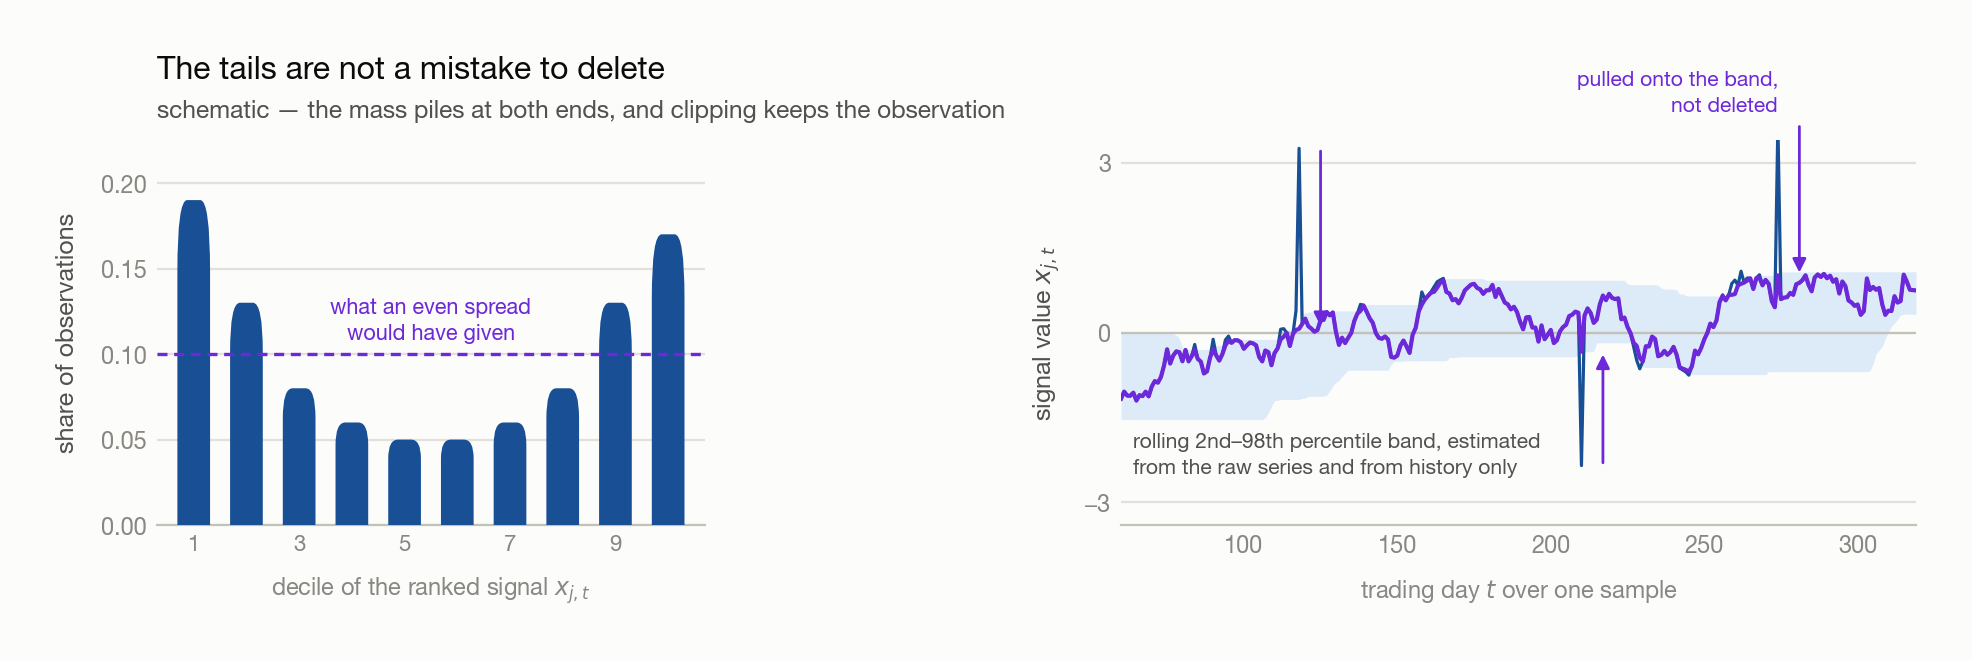
\includegraphics[width=\linewidth]{winsorize-band-light}
\end{figure}

Deleting the far points, which is the textbook move, fails twice here:

\begin{itemize}
  \item \textbf{The sample is already small.} Every deletion sharpens \S\ref{sec:defects}'s third
    defect, and in a messy sample it is not even clear which points are outliers.
  \item \textbf{The tail carries information.} What the book does when a signal goes extreme is
    exactly what the model should learn. Delete those dates and it never can.
\end{itemize}

\begin{definition}[Winsorization]
Replacing any value outside a chosen quantile band by the nearer edge of the band:
\[
  x^{\mathrm{clip}}_{j,t}
  = \min\!\left( \max\!\left( x_{j,t},\; Q^{\mathrm{lo}}_{j,t} \right),\; Q^{\mathrm{hi}}_{j,t} \right)
\]
where $Q^{\mathrm{lo}}_{j,t}$ and $Q^{\mathrm{hi}}_{j,t}$ are quantiles of signal $j$ over the
trailing $L$ dates --- 1 and 99 percent, or 2.5 and 97.5 percent; there is no canonical pair.
\end{definition}

\begin{note}[Compare raw to raw]
The band for date $t$ must be estimated from the \textbf{unclipped} history. Feed yesterday's
capped value into today's quantile and the band walks inward on itself, a little further every
step. Keep the raw column and produce the clipped one beside it.
\end{note}

\begin{note}[Why the band rolls]
A value that is extreme against the last three months may be unremarkable six months later, once
the market has moved to it. A fixed threshold pins such a signal at the 99th percentile forever; a
rolling one releases it as soon as the surrounding distribution catches up.
\end{note}

$\rightarrow$ \texttt{rolling}, \texttt{quantile} and \texttt{clip} as pandas calls:
\ch{08}{Toolbox}.

\subsection{Standardizing: put every signal on one scale}
\label{sec:standardize}

Momentum lives in roughly $[-0.05,\, 0.05]$. VIX lives in $[0,\, 100]$. Fit both and the
coefficients absorb the mismatch.

\begin{claim}
Coefficient magnitudes carry no information about a signal's importance until the signals share a
scale.
\end{claim}

\begin{proof}
Replace $x_j$ by $c\,x_j$ for some $c > 0$. The fitted values are unchanged if $\beta_j$ is
replaced by $\beta_j / c$, and least squares chooses fitted values --- so the fit is identical and
the coefficient is whatever the units make it. A comparison of $\beta$ magnitudes across
differently scaled signals is therefore a comparison of units.
\end{proof}

The consequence is not merely aesthetic. Every input is an \textbf{estimate} and carries error: a
momentum measured from returns is the residue of participants entering and leaving, and a jump in
it is as likely to be noise as news. A large $\beta$ multiplies that noise into the prediction,
while the small $\beta$ on the wide-ranging signal cannot respond when it genuinely moves.

\begin{definition}[Standardized signal]
\[
  z_{j,t} = \frac{x_{j,t} - \mu_j}{\sigma_j}
\]
with $\mu_j$ and $\sigma_j$ the mean and standard deviation of signal $j$ over the estimation
window. Dividing by a rolling standard deviation, or by a cross-sectional sum, are alternatives;
what matters is that \textbf{every signal is treated the same way}.
\end{definition}

\begin{figure}[h]
  \centering
  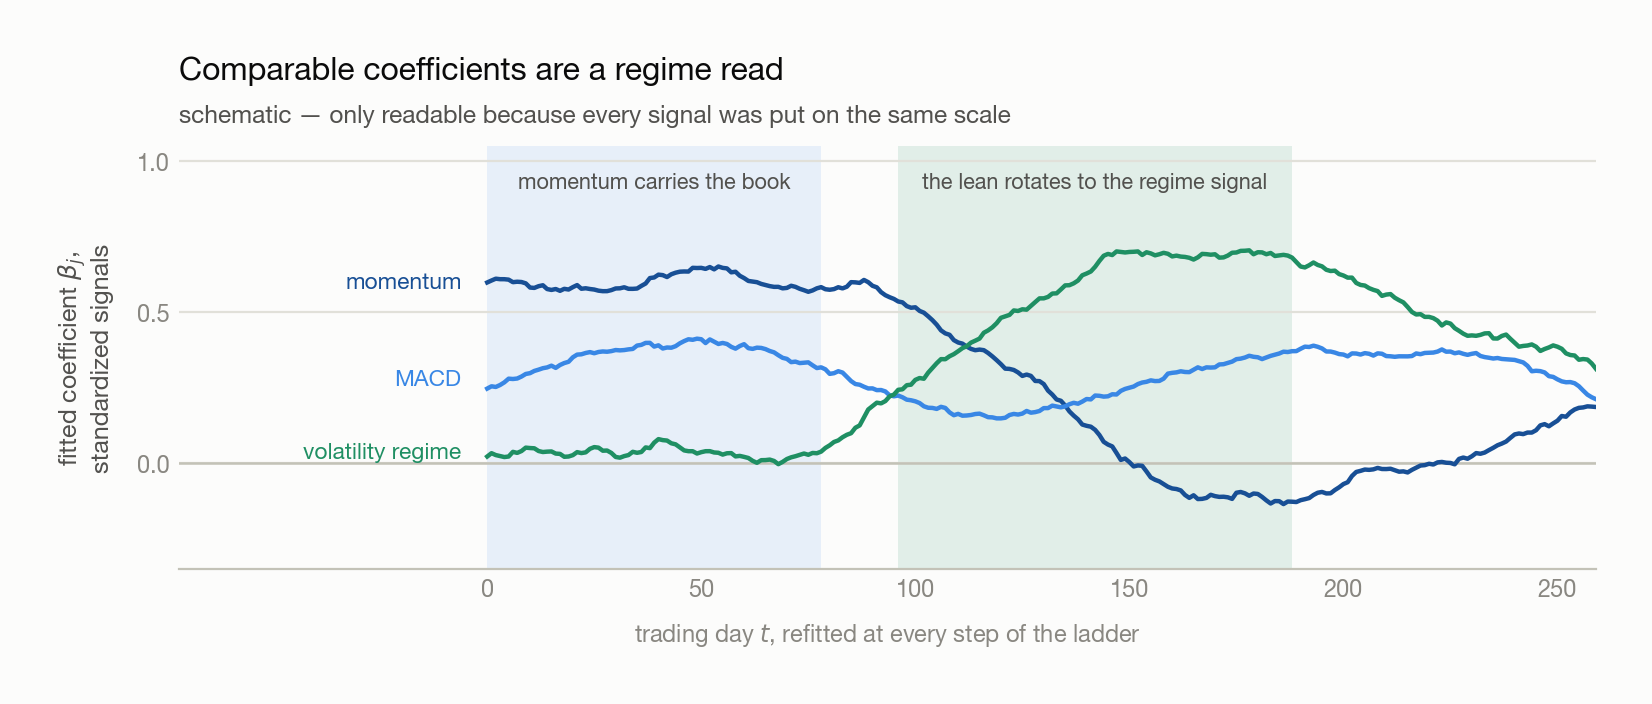
\includegraphics[width=\linewidth]{beta-paths-light}
\end{figure}

Three things follow, in increasing order of usefulness:

\begin{center}
\begin{tabularx}{\linewidth}{@{}L{4.4cm}X@{}}
\toprule
\textbf{Consequence} & \textbf{Why} \\
\midrule
Coefficients become comparable
& With units removed, $\beta_j$ measures response per standard deviation of signal --- the same
question for every signal. \\
\addlinespace
The coefficient path becomes a regime read
& Plot every $\beta_j$ from every rung on one axis. Momentum dominating one stretch and volatility
another \textbf{is} the change in market sentiment, in a form you can look at. \\
\addlinespace
Errors partly cancel
& On one scale, with comparable coefficients and errors that are close to independent across
signals, the noise in the combined prediction averages down as signals are added, instead of being
dominated by whichever signal has the largest units. \\
\bottomrule
\end{tabularx}
\end{center}

\subsection{Which mean and standard deviation you may use}
\label{sec:lookahead}

$\mu_j$, $\sigma_j$ and the quantile band all have to be estimated from somewhere, and that choice
is where look-ahead enters.

The rule follows from \textbf{where the model is built}: at the \emph{end} of the training window.
Every date inside that window is history at that moment, so standardizing with the whole training
window's mean and standard deviation is legitimate --- even though, from the point of view of an
individual date early in the window, the statistic used to scale it was computed partly from its
own future.

\begin{center}
\begin{tabularx}{\linewidth}{@{}L{6cm}X@{}}
\toprule
\textbf{At this point of construction} & \textbf{These statistics are available} \\
\midrule
End of the training window & the whole training window \\
End of the training window & \textbf{never} the validation segment, and never test \\
End of a refit window      & the whole refit sample, validation segment included \\
\bottomrule
\end{tabularx}
\end{center}

\begin{note}
The distinction is between \emph{a signal's} information set and \emph{the model's}. A signal
computed on date $t$ may use only data up to $t$, because it has to be computable live. The model
is not computed on date $t$; it is computed once, at the end of its window, and then applied
forward. Confusing the two costs either a leak or an estimate worse than the one you were entitled
to.
\end{note}

\begin{note}
This is the failure worth being paranoid about. In a time series the smallest leak makes the
result beautiful, and the gap between a beautiful backtest and the live book is where the money
goes.
\end{note}

% ============================================================================
\section*{Appendix · Notation}
\addcontentsline{toc}{section}{Appendix · Notation}

Throughout, $t$ is the date, $i$ indexes assets and $j$ indexes signals.

\begin{center}
\begin{tabularx}{\linewidth}{@{}L{4cm}XL{2.6cm}@{}}
\toprule
\textbf{Symbol} & \textbf{Means} & \textbf{First used} \\
\midrule
$x_{j,t}$, $x^{\mathrm{clip}}_{j,t}$, $z_{j,t}$
& signal $j$ on date $t$: raw, after clipping, after standardizing
& \S\ref{sec:rung}, \S\ref{sec:clip}, \S\ref{sec:standardize} \\
\addlinespace
$y_t$, $\beta_j$
& the forward return being predicted, and the coefficient the fit puts on signal $j$
& \S\ref{sec:rung} \\
\addlinespace
$X$, $y$, $b$, $n$, $p$, $s^2$
& the design matrix, the response, the estimated coefficients, the number of dates, the number of
signals, the residual variance estimate
& \S\ref{sec:duplication} \\
\addlinespace
$\lambda$
& the $L_1$ penalty strength --- searched on a grid, not fitted
& \S\ref{sec:rung} \\
\addlinespace
$L$
& the trailing window, in dates, that the clip band is estimated over
& \S\ref{sec:clip} \\
\addlinespace
$Q^{\mathrm{lo}}_{j,t}$, $Q^{\mathrm{hi}}_{j,t}$
& the low and high quantiles of that window
& \S\ref{sec:clip} \\
\addlinespace
$\mu_j$, $\sigma_j$
& the mean and standard deviation used to standardize signal $j$
& \S\ref{sec:standardize} \\
\addlinespace
$w_i$, $\gamma$, $E[r_p]$
& the portfolio weight on asset $i$, the risk-aversion coefficient, and the portfolio's expected
return
& \S\ref{sec:optimizer} \\
\bottomrule
\end{tabularx}
\end{center}

\begin{note}[Collisions to watch]
$\sigma_j$ here is one \textbf{signal's} dispersion, used only to rescale it --- not
\ch{02}{Testing a Signal}'s $\sigma_{s,t}$, an asset's trailing volatility, and not
\ch{04}{Volatility Regimes}'s $\sigma$, the amplitude of the tape. $\beta_j$ is a coefficient on a
\textbf{signal}, as in \ch{04}{Volatility Regimes}, never a market beta. $\lambda$ is the penalty
and $\gamma$ the risk aversion: the lecture wrote both as $\lambda$ and then renamed the second,
and they are unrelated. $L$ is a trailing window as in \ch{04}{Volatility Regimes}, here over a
signal rather than over returns.
\end{note}

% ============================================================================
\section*{Common pitfalls}
\addcontentsline{toc}{section}{Common pitfalls}

\begin{center}
\begin{tabularx}{\linewidth}{@{}L{5.2cm}X@{}}
\toprule
\textbf{Belief} & \textbf{Correction} \\
\midrule
``More rows will fix the small sample.''
& Duplicating them changes no coefficient and shrinks the standard errors by $\sqrt{2}$ ---
\S\ref{sec:duplication}. Score more of the dates you have instead. \\
\addlinespace
``Outliers are contamination; drop them.''
& They are the dates you most want the model to have seen. Clip them onto a rolling band ---
\S\ref{sec:clip}. \\
\addlinespace
``Clip against the series I am building.''
& The band must come from the raw history, or it walks inward on itself --- \S\ref{sec:clip}. \\
\addlinespace
``Standardizing with the whole training window is look-ahead.''
& The model is constructed at the end of that window, so the window is history to it. Using the
\emph{validation} segment is the leak --- \S\ref{sec:lookahead}. \\
\addlinespace
``The validation block is a second test set.''
& It chooses the model class, $\lambda$, $\gamma$ and the cap. Everything it chooses on, it has
been fitted to. \\
\addlinespace
``A bigger $\beta$ means a more important signal.''
& Only after \S\ref{sec:standardize}. Before it, $\beta$ is a statement about units. \\
\bottomrule
\end{tabularx}
\end{center}

% ============================================================================
\section*{Open questions}
\addcontentsline{toc}{section}{Open questions}

\begin{itemize}
  \item \textbf{Rolling or expanding train?} The ladder above drops the oldest segment each step.
    Keeping it gives more data at the cost of holding on to regimes that have gone.
  \item \textbf{How long is a segment, really?} Two to three months is asserted from how fast a
    crowd changes its mind, not measured. It could be estimated --- from how quickly fitted
    coefficients decay.
  \item \textbf{Does $\gamma$ survive?} It is tuned on the outer block. Nothing yet says a risk
    appetite chosen in one regime is the right one in the next.
\end{itemize}

\bigskip
\hrule
\bigskip

% ============================================================================
\section*{Next $\rightarrow$ Backtest Prototype --- Implementation Notes}
\addcontentsline{toc}{section}{Next → Backtest Prototype}

Before moving on, \textbf{build the ladder end to end and put the simplest possible model in it}:
cut the sample into 63-day segments, run three-train / one-validation / one-test frames forward,
clip and standardize every signal inside each rung, and fit one Lasso. Report, per rung, how many
features survived and what the test IC was --- then plot every $\beta_j$ against time, which is
\S\ref{sec:standardize}'s figure drawn from your own numbers rather than from an illustration.
Choose $\lambda$, $\gamma$ and the cap only after that runs.

Expect the result to be weak. A single public signal that was strongly significant would be a
signal nobody else had, which is not the situation --- see the lecture note below for why that is
the correct outcome rather than a bug.

$\rightarrow$ The lecture this chapter is drawn from, including the market history behind it:
\textit{Walk-Forward Modelling, Winsorization, and Standardization}.

You should be able to explain:

\begin{itemize}[label=\tickbox]
  \item Why a single split ignores time, and why one year of validation is not a risk estimate
  \item What duplicating the sample does to the coefficients and to their standard errors
  \item Why each rung's test segment is the next rung's validation segment
  \item Which decisions belong to the validation segment, which to the held-out block, and which
    to neither
  \item Why an outlier is clipped rather than deleted, and why the band is computed from the raw
    series
  \item Why coefficients are meaningless across signals of different scale, and what the
    coefficient paths show once they are not
\end{itemize}

\end{document}
